\documentclass[11pt]{beamer}

\usetheme{metropolis}

\usepackage{graphicx}
\usepackage{physics}
\usepackage{adjustbox}
\usepackage{caption}
\usepackage{chemformula}
\usepackage{quoting}
\usepackage{multicol}
\usepackage[style=chem-angew,backend=bibtex]{biblatex}
\bibliography{references}
%
% Choose how your presentation looks.
%
% For more themes, color themes and font themes, see:
% http://deic.uab.es/~iblanes/beamer_gallery/index_by_theme.html
%
\mode<presentation>
{
  \usetheme{default}      % or try Darmstadt, Madrid, Warsaw, ...
  \usecolortheme{default} % or try albatross, beaver, crane, ...
  \usefonttheme{default}  % or try serif, structurebold, ...
  \setbeamertemplate{navigation symbols}{}
  \setbeamertemplate{caption}[numbered]
  \setbeamerfont{footnote}{size=\tiny}
} 

\usepackage[english]{babel}
\usepackage[utf8]{inputenc}
\graphicspath{{image/}}

\AtBeginSection[]{
\begin{frame}{Outline}
  \tableofcontents[currentsection]
\end{frame}
}

\title{Chapter 3: Chemical Compounds}
\institute{Chemistry Department, Cypress College}
\date{Sept 12, 2022}

\begin{document}

\begin{frame}
  \titlepage
\end{frame}

\begin{frame}{Lecture and Lab Weekly Agenda}
  \textbf{Lab Section}

  \begin{itemize}
  \item Lab Safety Quiz
  \item Begin Exp 2 - Nomenclature
  \end{itemize}

  \textbf{Lecture Section}

  \begin{itemize}
  \item Go over homework assignment; present your work
    for 1pt EC
  \item Review Ch 3+8 - Chemical Compounds and Types of Bonding
  \item Finish up Ch 3 lect and worksheet
  \item Homework and quiz 3 released Fri, Sept 16 at 3pm
  \item Homework due Fri, Sept 23 at 11:59pm
  \item Quiz 3 due Mon, Sept 19 at 11:59pm
  \end{itemize}
\end{frame}

\section{Review: Electronegativity of Ionic and Molecular Compounds}

\begin{frame}{Introduction to Bonding}
  \textbf{Ionic Bonding}
  \begin{itemize}
  \item Electrons transferred from metal
    to nonmetal
  \item Ionized atoms and electrostatic interactions
  \end{itemize}

  \textbf{Covalent Bonding (CB)}
  \begin{itemize}
  \item Sharing of electrons between atoms (usually
    look at as pairs)
  \item Generally occurs between nonmetals in molecular
    elements, molecular compounds, and polyatomic ions
  \end{itemize}
\end{frame}

\begin{frame}{Consideration of Electronegativity}
  \centering
  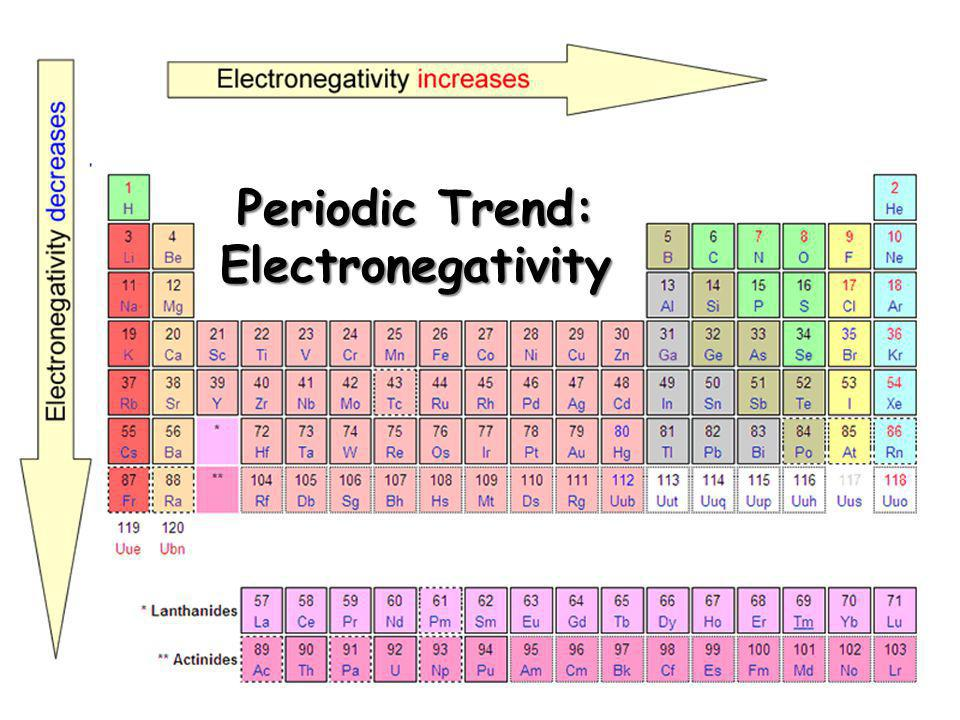
\includegraphics[width=\linewidth]{electronegativity}
\end{frame}


\begin{frame}{Practice: Ionic or Molecular compounds?}
  \textbf{Determine whether the following compounds are ionic or molecular.}
  \begin{multicols}{2}
  \begin{itemize}
  \item Cl$_2$CO
  \item MnO
  \item NCl$_3$
  \item CoBr$_2$
  \item K$_2$S
  \item CO
  \item CaF$_2$
  \item HI
  \item CaO
  \item IBr
  \item CO$_2$
  \item C$_6$H$_{12}$O$_6$ (sugar)
  \end{itemize}
  \end{multicols}
\end{frame}

\begin{frame}{Practice: Polarity}
  \textbf{Which of the following is the most polar bond?}

    C--C; C--H; N--H; O--H; F--H; Se--H
\end{frame}

\begin{frame}{Monoatomic and Polyatomic Ions}
  \centering
  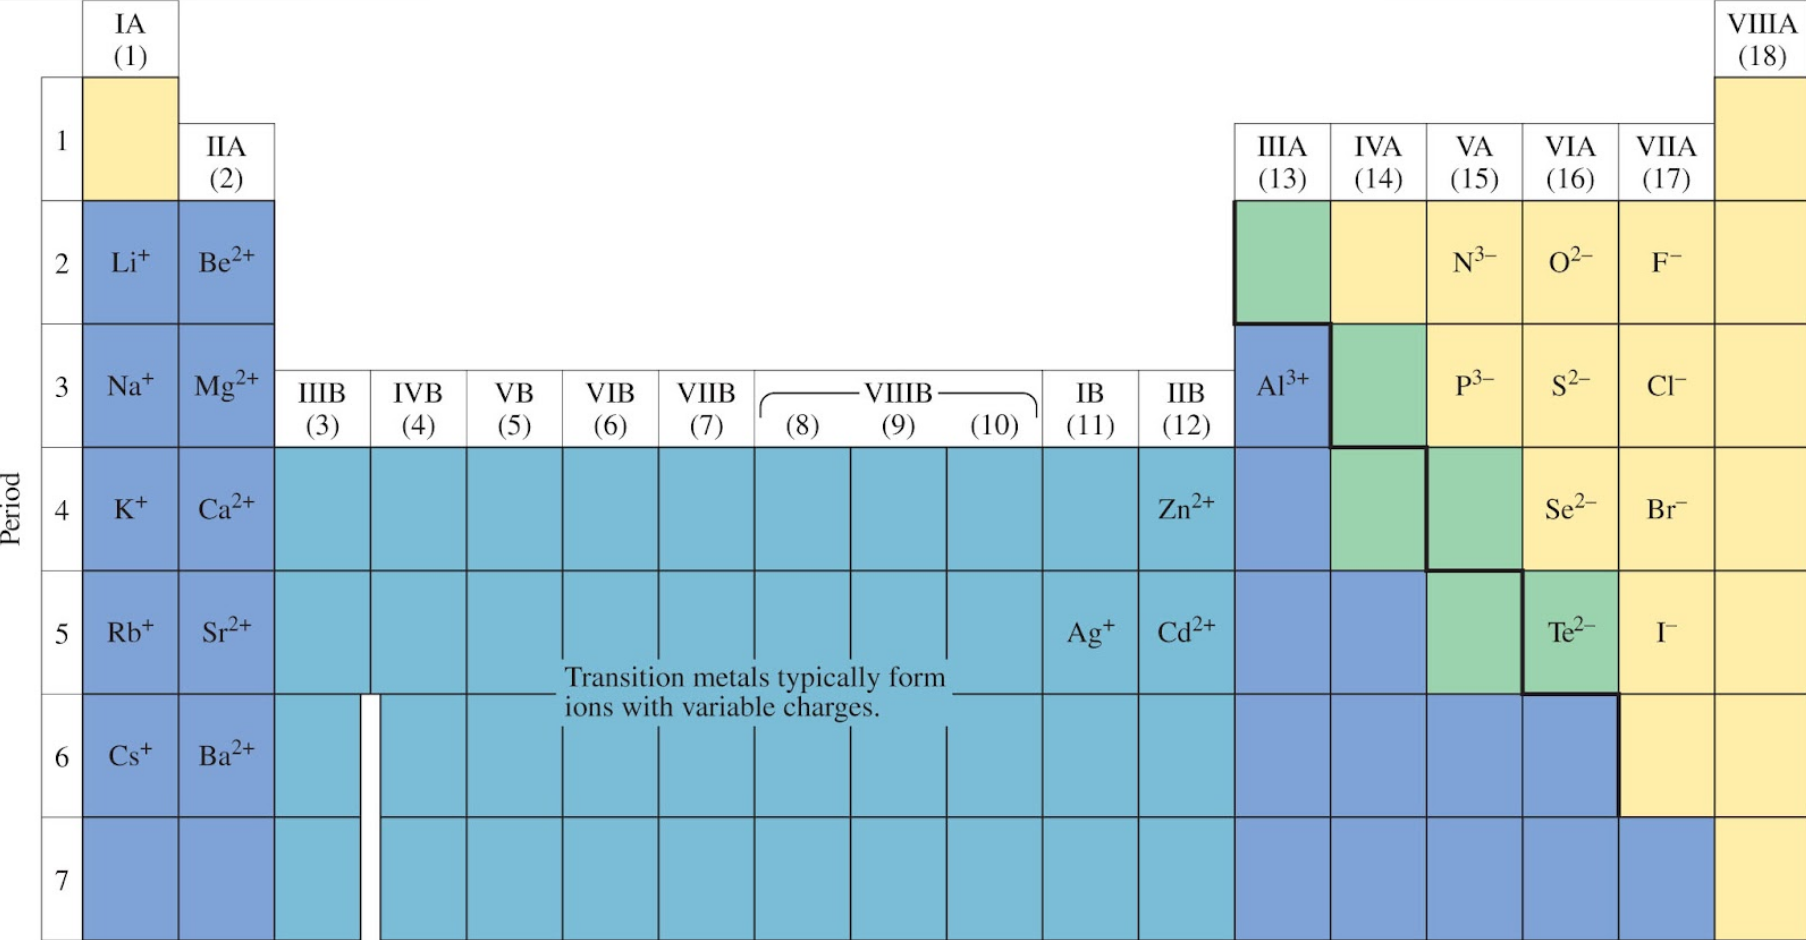
\includegraphics[width=\linewidth]{monoatomic_ion}
\end{frame}

\begin{frame}{Monoatomic and Polyatomic Ions}
  \centering
  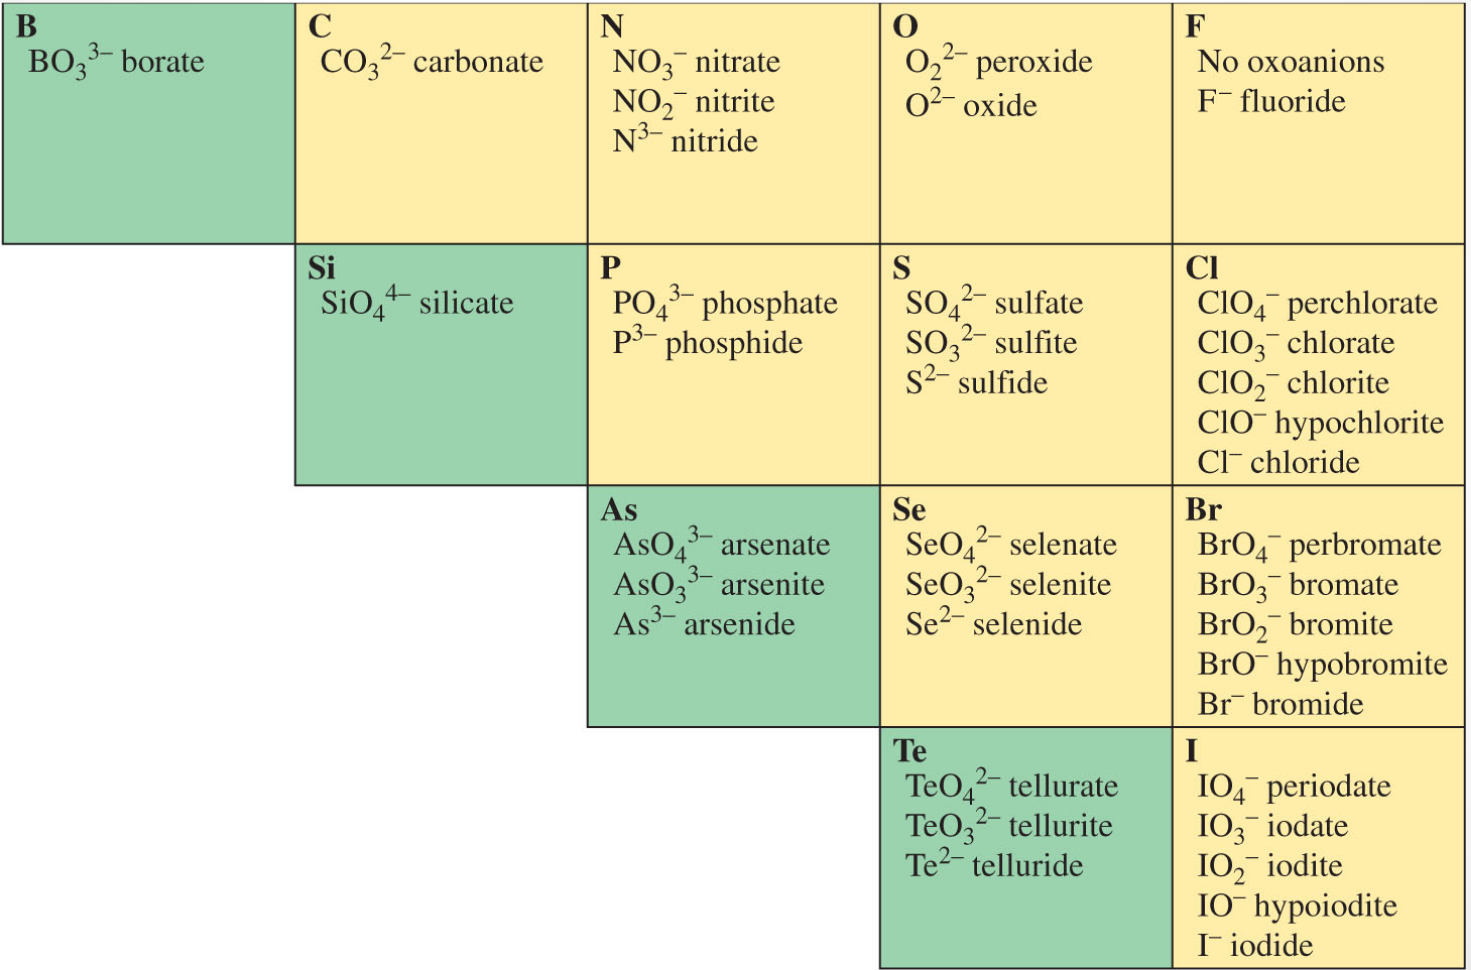
\includegraphics[width=\linewidth]{polyatomic_ion}
\end{frame}

\begin{frame}{Additional Polyatomic Ions}
  \centering
  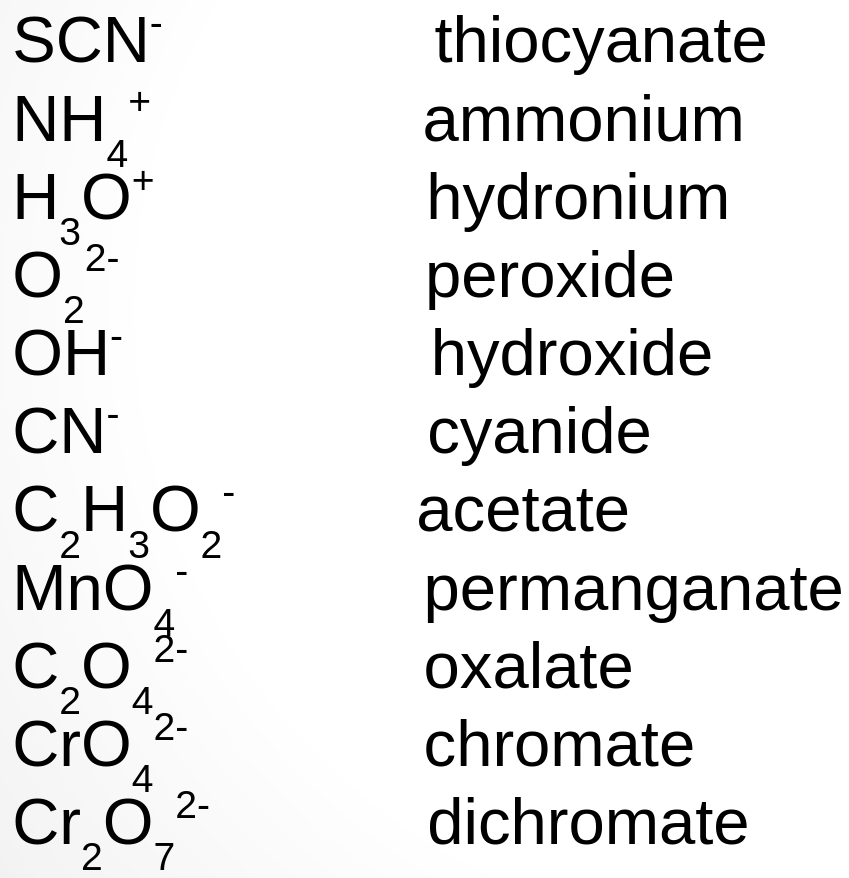
\includegraphics[width=0.7\linewidth]{more_poly_ions}
\end{frame}

\section{Naming Molecular Compounds}

\begin{frame}{Naming Molecular Compounds}
  \begin{center}
    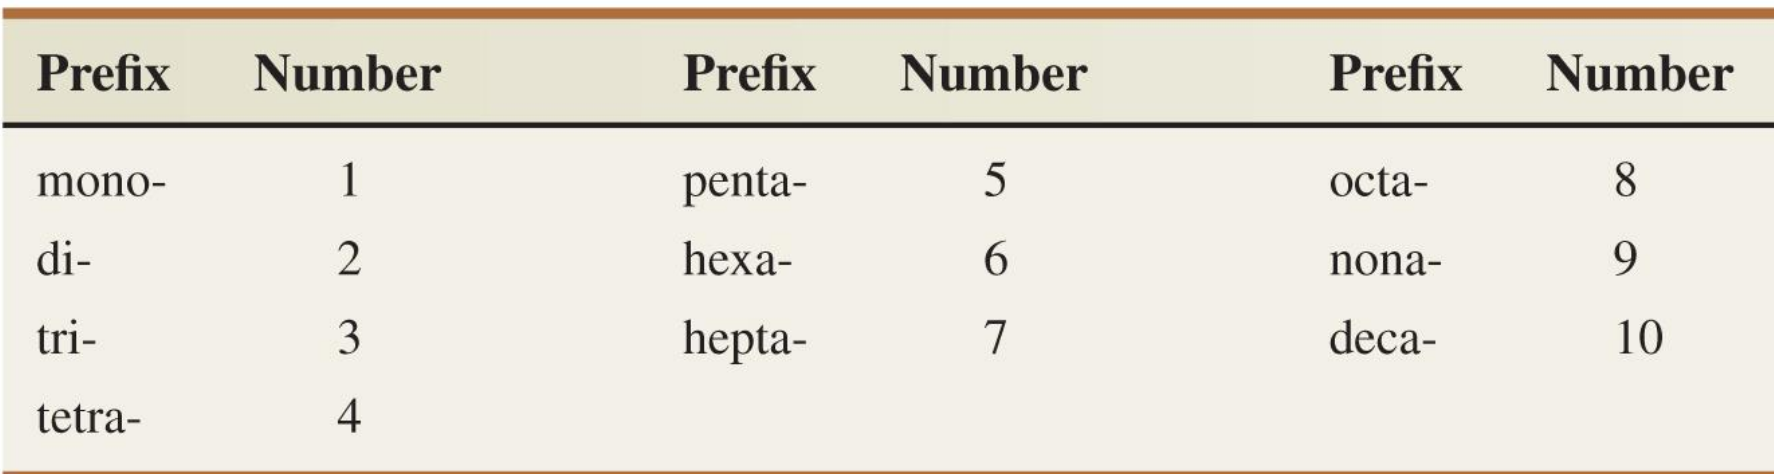
\includegraphics[width=\linewidth]{prefix_name}
  \end{center}
  
  \begin{enumerate}
  \item Use numerical prefix for the element (usually ignore the first
    when using ``mono'')
  \item Add ``-ide'' to the second element
  \end{enumerate}
\end{frame}

\begin{frame}{Naming Binary Molecular Compounds}
  \begin{itemize}
  \item H$_2$O
  \item N$_2$O$_4$
  \item CO
  \item CH$_4$
  \end{itemize}
\end{frame}

\subsection{Acids and Bases}

\begin{frame}{Naming Acids and Bases}
  \begin{center}
    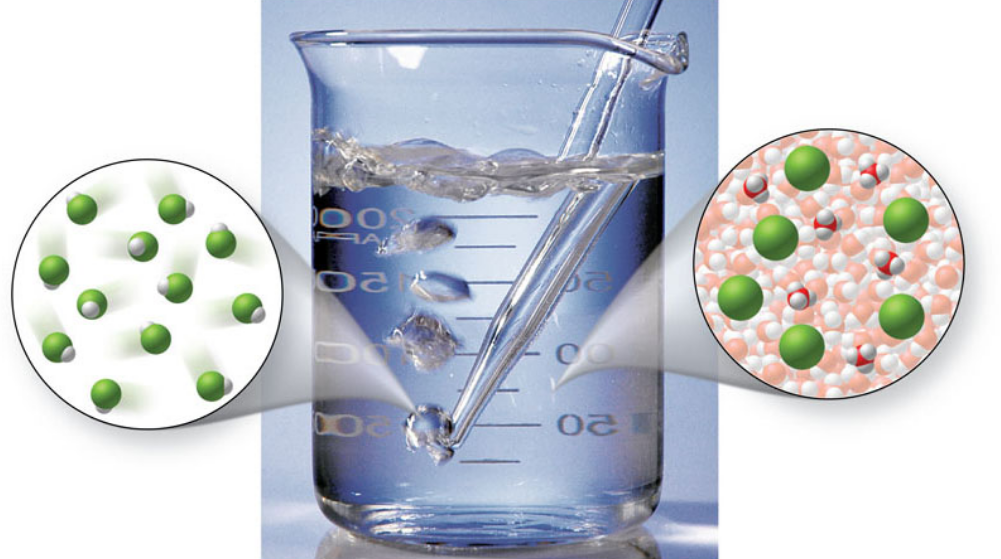
\includegraphics[width=0.5\linewidth]{acid_base}
  \end{center}

  \begin{enumerate}
  \item If anion ends in ``-ide,'' add ``hydro'' before the
    root of the anion name followed by ``-ic acid''
  \item If anion ends in ``-ate,'' use the root of the anion
    name followed by ``-ic acid''
  \item If anion ends in ``-ite,'' use the root of the anion
    name followed by ``-ous acid''
  \end{enumerate}
\end{frame}

\begin{frame}{Practice: Naming the Acid}
  \begin{itemize}
  \item HCl
  \item HNO$_3$
  \item H$_2$CO$_3$
  \item H$_2$SO$_3$
  \end{itemize}
\end{frame}

\begin{frame}{Definition(s) of an Acid}
  \textbf{Arrhenius Acid} - dissociation of acid in water to yield
  the ions e.g. HCl(aq) $\rightarrow$ H$^+$(aq) + Cl$^-$(aq)
  
  \textbf{Br{\o}nsted Acid} - any species that can donate a proton
  H$^+$

  \textbf{Lewis Acid} - donation of a pair of electrons
\end{frame}

\end{document}
